% Created 2023-01-12 Πεμ 22:29
% Intended LaTeX compiler: pdflatex
\documentclass[11pt]{article}
\usepackage[utf8]{inputenc}
\usepackage[T1]{fontenc}
\usepackage{graphicx}
\usepackage{longtable}
\usepackage{wrapfig}
\usepackage{rotating}
\usepackage[normalem]{ulem}
\usepackage{amsmath}
\usepackage{amssymb}
\usepackage{capt-of}
\usepackage{hyperref}
\usepackage{booktabs}
\usepackage{import}
\usepackage[LGR, T1]{fontenc}
\usepackage[greek, english]{babel}
\usepackage{alphabeta}
\usepackage{esint}
\usepackage{mathtools}
\usepackage{esdiff}
\usepackage{makeidx}
\usepackage{glossaries}
\usepackage{newfloat}
\usepackage{minted}
\usepackage{chemfig}
\usepackage{svg}
\usepackage[a4paper, margin=3cm]{geometry}
\author{Βιδιάνος Γιαννίτσης}
\date{\today}
\title{Ανάλυση του block 400 - Παραγωγή Γλυκερόλης}
\hypersetup{
 pdfauthor={Βιδιάνος Γιαννίτσης},
 pdftitle={Ανάλυση του block 400 - Παραγωγή Γλυκερόλης},
 pdfkeywords={},
 pdfsubject={},
 pdfcreator={Emacs 28.2 (Org mode 9.5.5)}, 
 pdflang={English}}
\makeatletter
\newcommand{\citeprocitem}[2]{\hyper@linkstart{cite}{citeproc_bib_item_#1}#2\hyper@linkend}
\makeatother

\usepackage[notquote]{hanging}
\begin{document}

\maketitle
\tableofcontents

\renewcommand{\abstractname}{Περίληψη}
\renewcommand{\tablename}{Πίνακας}
\renewcommand{\figurename}{Σχήμα}
\renewcommand\listingscaption{Κώδικας}

\section{Διάγραμμα ροής και επεξήγηση}
\label{sec:org8f5951f}
\begin{figure}[htbp]
\centering
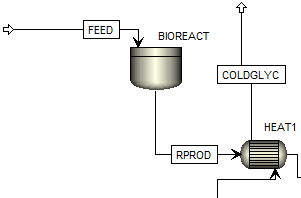
\includegraphics[width=.9\linewidth]{Διάγραμμα_ροής_και_Επεξήγηση/2023-01-12_16-53-41_screenshot.png}
\caption{Διάγραμμα ροής του block 400}
\end{figure}

Στο block 400 όπως προαναφέρθηκε γίνεται η παραγωγή της γλυκερόλης, ενός από τα δύο βασικά προιόντα στον βιοαντιδραστήρα, του οποίου το προιόν προθερμαίνεται με το ρεύμα της καθαρής γλυκερόλης του block 500. Στο διάγραμμα ροής φαίνονται ο βιοαντιδραστήρας και ο εναλλάκτης θερμότητας που απαιτούνται.

\section{Σχεδιαστικές Επιλογές}
\label{sec:org1e50cce}
Η βασική σχεδιαστική επιλογή του block αυτού είναι ο τύπος και η λειτουργία του βιοαντιδραστήρα. Για τον εναλλάκτη δεν χρειάζεται να αναφερθεί κάτι καθώς ο σκοπός του είναι βασικά να ψύξει την παραγόμενη γλυκερόλη, το οποίο μπορεί να γίνει ταυτόχρονα με την προθέρμανση του ρεύματος εξόδου του αντιδραστήρα, άρα ήταν μία εύκολη επιλογή που βοηθάει στην ενεργειακή ολοκλήρωση της διεργασίας.

Για τον αντιδραστήρα, ο τύπος που επιλέχθηκε είναι ο αντιδραστήρας RBatch. Αυτό έγινε διότι η λειτουργία διαλείποντος έργου είναι αρκετά διαδεδομένη στους βιοαντιδραστήρες για 2 βασικούς λόγους. Ο πρώτος είναι πως οι αντιδράσεις αυτές έχουν αυτοκαταλυτική φύση άρα σε μία διάταξη συνεχούς ροής, υπάρχει βιομάζα στην έξοδο του αντιδραστήρα αντί να συσσωρεύεται όλη στον αντιδραστήρα, το οποίο μειώνει τον ρυθμό αντίδρασης, ενώ ο δεύτερος είναι ότι σε μία μικροβιακή καλλιέργεια, η οποία λειτουργεί σε μόνιμες συνθήκες, υπάρχει πάντα η πιθανότητα επιμόλυνσης του αντιδραστήρα. Στις περισσότερες περιπτώσεις, η επιμόλυνση αυτή δεν θα δράσει βοηθητικά για τον μικροοργανισμό μας και θα μειώσει τον ρυθμό της αντίδρασης και πιθανότατα την καθαρότητα του προιόντος. Όταν παρατηρηθεί κάτι τέτοιο, θα πρέπει να γίνει ολικό shut down του αντιδραστήρα και να καθαριστεί, το οποίο αποτελεί ένα μεγάλο διάστημα μη παραγωγικού χρόνου μέχρι να ξαναρχίσει το σύστημα σε μόνιμη κατάσταση. Στην περίπτωση του batch αντιδραστήρα, αυτός καθαρίζεται σε κάθε batch και λειτουργεί σε μη μόνιμη κατάσταση, άρα δεν χάνεται χρόνος για την αποκατάσταση της μόνιμης κατάστασης. Επίσης, είναι σημαντικά μικρότερη η πιθανότητα επιμόλυνσης.

Επιπλέον, ένας αντιδραστήρας CSTR πρέπει να λειτουργεί σε τέτοιες συνθήκες ώστε να μην οδηγηθεί σε μόνιμη κατάσταση έκπλυσης, κάτι το ανεπιθύμητο. Αυτό σημαίνει, πως για την τροφοδοσία του αντιδραστήρα μας, ο όγκος που απαιτείται είναι τουλάχιστον 3 φορές μεγαλύτερος αυτού του batch και αυτό είναι χωρίς να ληφθεί υπόψην η αργή κινητική, λόγω της οποίας ο όγκος μπορεί να είναι ακόμη μεγαλύτερος. Θεωρητικά, αυτό θα μπορούσε να λυθεί σε έναν αντιδραστήρα PFR, όμως η ανάδευση είναι ιδιαίτερα σημαντική στις αερόβιες μικροβιακές καλλιέργειες καθώς βοηθάει στην ομοιογένεια και στην συνεχή αιώρηση της βιομάζας, παράγοντες που επιτρέπουν την γρηγορότερη ανάπτυξη της. Επίσης, βελτιώνεται η διασπορά του δυσδιάλυτου οξυγόνου το οποίο πρέπει να υπάρχει και σε ορισμένες περιπτώσεις η μεταφορά του είναι από τα πιο βραδέα στάδια της διεργασίας. Για αυτό, οι αντιδραστήρες PFR δεν προτιμούνται συνήθως για τέτοιες διεργασίες, εκτός από ορισμένες περιπτώσεις κλινών στις οποίες υπάρχει ακινητοποιημένη βιομάζα, μία διεργασία η οποία είναι ιδιαίτερα περίπλοκη στην μελέτη της.

Όλοι αυτοί είναι λόγοι για τους οποίους δεν προτιμάται ένα σύστημα συνεχούς ροής, ακόμη και στην περίπτωση που θέλουμε πολύ υψηλή παραγωγικότητα στον αντιδραστήρα.

Για τις συνθήκες λειτουργίας του, εφόσον έχουμε μία καθαρή καλλιέργεια ενός μικροοργανισμού, οι βέλτιστες συνθήκες λειτουργίας είναι αυστηρά καθορισμένες από τον μικροοργανισμό και είναι τυπικά σε ένα στενό εύρος τιμών το οποίο βρίσκεται από βιβλιογραφία. Για τον μικροοργανισμό Candida glycerinogenes ο οποίος έχει χρησιμοποιηθεί στην διεργασία αυτή, βρέθηκε βιβλιογραφικά πως η βέλτιστη συγκέντρωση γλυκόζης είναι 230-250 g/l, η συγκέντρωση ουρίας 2 g/l, η συγκέντρωση φωσφόρου 55-60 mg/l (προστίθεται στην μορφή του corn steep liquor με βάση την βιβλιογραφία), το pH μεταξύ 4-6 και η θερμοκρασία μεταξύ 29 και 33 \(^oC\) \textsuperscript{\citeprocitem{1}{1}} . Για τα θρεπτικά συστατικά, βρέθηκε η ποσότητα νερού που απαιτείται για την παραγωγή διαλύματος γλυκόζης 230 g/l με όλη την γλυκόζη της διεργασίας και έπειτα η ποσότητα ουρίας και corn steep liquor (CSL) που απαιτείται ώστε οι συγκεντρώσεις τους να είναι οι επιθυμητές. Το pH δεν χρειάζεται να ρυθμιστεί σε κάποιο επίπεδο καθώς παρουσία του CSL το pH είναι στην επιθυμητή περιοχή ενώ η θερμοκρασία ρυθμίστηκε στους 30 \(^oC\) καθώς για αυτή την τιμή υπάρχουν κινητικά δεδομένα \textsuperscript{\citeprocitem{2}{2}} . Το CSL δεν προστέθηκε στην προσομοίωση της διεργασίας καθώς δεν υπάρχει στην βάση δεδομένων του Aspen και η πολυπλοκότητα της διεργασίας θα αυξανόταν σημαντικά με την προσθήκη του.

\section{Υπολογισμοί}
\label{sec:orgf0f5ee4}
Οι βασικοί υπολογισμοί του block 400 είναι 3. Η στοιχειομετρία της μικροβιακής αντίδρασης, η οποία δεν είναι γνωστή εξ'αρχής, η κινητική της μικροβιακής αντίδρασης και οι υπολογισμοί του εναλλάκτη. Οι υπολογισμοί του εναλλάκτη έγιναν απευθείας στο Aspen για αυτό θα επεξηγηθούν περισσότερο στην προσομοίωση. Για την στοιχειομετρία και την κινητική της μικροβιακής αντίδρασης, βασιστήκαμε σε πειραματικά δεδομένα \textsuperscript{\citeprocitem{1}{1},\citeprocitem{2}{2}} . Ο προσδιορισμός της στοιχειομετρίας της αντίδρασης είναι μία περίπλοκη διαδικασία, ειδικά επειδή δεν είναι γνωστός εκ των προτέρων ο τύπος της βιομάζας. Υπάρχουν διάφορες τεχνικές που μπορούν να ακολουθηθούν για τον προσδιορισμό αυτόν, αλλά αποφασίστηκε πως αντί να υποτεθεί ο μοριακός τύπος της βιομάζας και να προκύψει μία αυθαίρετη μικροβιακή αντίδραση, να υπολογιστούν όσοι συντελεστές μπορούν με βάση τα πειραματικά δεδομένα για τα yields της αντίδρασης και να υπολογιστούν από αυτά ο τύπος της βιομάζας και όσοι στοιχειομετρικοί συντελεστές δεν είναι πειραματικά γνωστοί. Η αναλυτική επεξήγηση των υπολογισμών αυτών παρατίθεται στο παράρτημα Γ. Προκύπτει πως η αντίδραση είναι η

\[ 1.22 S + 0.24U + 2.89 O_2 \rightarrow 0.45 C_{1.48}H_{2.95}O_{0.048}N_{0.11} + G + 0.025E + 0.019Ac + 3.5CO_2 + 2.5H_2O \]
όπου S η γλυκόζη (υπόστρωμα), U η ουρία, G η γλυκερόλη, Ε η αιθανόλη και Ac το οξικό οξύ.

Για την κινητική της μικροβιακής αντίδρασης, έγινε προσαρμογή των παραπάνω πειραματικών δεδομένων στο μοντέλο Monod, το οποίο είναι το πιό κλασσικό μοντέλο για την μικροβιακή ανάπτυξη. Το πραγματικό κινητικό μοντέλο ενδέχεται να είναι πιό περίπλοκο από αυτό, αλλά απουσία μίας ολοκληρωμένης κινητικής μελέτης, το μοντέλο Monod είναι μία καλή πρώτη προσέγγιση. Ο ρυθμός με βάση το μοντέλο Monod είναι ο ρυθμός ανάπτυξης της βιομάζας. Με βάση την στοιχειομετρία όμως, ο ρυθμός της αντίδρασης ο οποίος θα χρησιμοποιηθεί στην διαστασιολόγηση του αντιδραστήρα θα είναι ο \(\frac{1}{0.45} \frac{dx}{dt}\).

Με βάση τα δεδομένα αυτά, το κινητικό μοντέλο που προέκυψε είναι το εξής:
\[ \frac{dx}{dt} = \frac{3.06*10^{-6}[S]}{236.19+[S]}[x] \] όπου οι σταθερές μ\textsubscript{max} και K\textsubscript{s} είναι υπολογισμένες σε μονάδες SI και οι συγκεντρώσεις σε g/l. Η προσαρμογή έγινε μέσω του Excel, το οποίο αρχείο μπορεί να βρεθεί \href{https://github.com/Vidianos-Giannitsis/Process-Design/blob/master/Calculations/c\_glycerinogenes\_kinetics.ods}{εδώ}.

\section{Προσομοιώσεις στο Aspen}
\label{sec:orgcf00b0e}
Το μοντέλο που χρησιμοποιήθηκε για την προσομοίωση είναι το NRTL-HOC. Το μοντέλο NRTL είναι ένα από τα πιο σύνηθη μοντέλα συντελεστών ενεργότητας, το οποίο είναι κατάλληλο για χημικά συστήματα σε χαμηλή πίεση. Η τροποποίηση των Hayden O' Connell στο μοντέλο αυτό χρησιμοποιείται όταν υπάρχουν μικρά οργανικά οξέα στο διάλυμα. Τα οξέα αυτά έχουν την ιδιαιτερότητα να μπορούν να αλληλεπιδράσουν μεταξύ τους με δεσμούς υδρογόνου στην αέρια φάση ακόμη και σε χαμηλές πιέσεις. Λόγω αυτών των αλληλεπιδράσεων, η αέρια φάση δεν μπορεί να θεωρηθεί ιδανική και για αυτό απαιτείται κάποια διόρθωση στο μοντέλο NRTL, την οποία πετυχαίνουν μοντέλα όπως το NRTL-HOC.

Το ρεύμα εισόδου της διεργασίας ορίστηκε με βάση τις συγκεντρώσεις που αναφέρθηκαν παραπάνω ως βέλτιστες. Έπειτα, ορίστηκε νερό ως ο διαλύτης σε μία ποσότητα τέτοια ώστε να υπάρχει όση γλυκόζη στο ρεύμα όση πρέπει να υπάρχει με βάση το block 200. Για τον βιοαντιδραστήρα, ορίστηκε ότι θα λειτουργεί σε σταθερή πίεση και θερμοκρασία (30 \(^oC\), 1 bar), με χρόνο λειτουργίας 80 ώρες (ο χρόνος που υπήρχε στα πειραματικά δεδομένα).

Το πιό ενδιαφέρον κομμάτι του βιοαντιδραστήρα είναι ότι μόλις βρούμε (με βάση την στοιχειομετρία και τα πειραματικά δεδομένα όπως περιγράφηκε παραπάνω) την βιομάζα του μικροοργανισμού, πρέπει αυτή να προσομοιωθεί στο Aspen. Η λογική που ακολουθήθηκε είναι η ίδια με αυτή που φαίνεται στο παράρτημα Β για την προσομοίωση της κυτταρίνης και της λιγνίνης ως conventional solids. Στην ίδια πηγή \textsuperscript{\citeprocitem{3}{3}} αναφέρεται και η προσομοίωση μίας βιομάζας, για αυτό με κάποιους υπολογισμούς, μπορούν εύκολα να υπολογιστούν τα χαρακτηριστικά της βιομάζας. Οι αναλυτικοί υπολογισμοί αυτοί φαίνονται στο παράρτημα Δ.

Για την κινητική, ορίστηκε η παραπάνω στοιχειομετρία, ενώ για την προσομοίωση του μοντέλου Monod, μπορεί να χρησιμοποιηθεί το μοντέλο LHHW με k=1, E=0, driving force τον αριθμητή του μοντέλου Monod και adsorption των παρανομαστή του. Αξίζει να αναφερθεί πως πρέπει οι μονάδες να είναι σε SI (όπως είναι στην προκειμένη περίπτωση) και στο Aspen πρέπει να μπούν οι λογάριθμοι των σταθερών και όχι οι ίδιες οι σταθερές. Επίσης, πρέπει να επιλεγεί το [C\textsubscript{i}] basis στο μενού του driving force ως mass concentration για να έχουν οι συγκεντρώσεις τις σωστές μονάδες.

Για τον εναλλάκτη του block, πρακτικά μας ενδιαφέρει να ψύξουμε το ρεύμα της καθαρής γλυκερόλης καθώς έτσι και αλλιώς δεν θα επαρκέσει για να φτάσει το ρεύμα την επιθυμητή θερμοκρασία. Για αυτό ψάχνουμε την χαμηλότερη θερμοκρασία που μπορούμε να πάμε το ρεύμα, η οποία προκύπτει πως είναι 44 \(^oC\), δηλαδή ένα ΔΤ = 14 \(^oC\) από την είσοδο του ψυχρού. Τα προιόντα του αντιδραστήρα είναι σε αρκετά μεγαλύτερη παροχή από ότι το ρεύμα αυτό, για αυτό στην αρχή του block 500 ολοκληρώνεται η θέρμανση αυτή.

\section{Παράρτημα Γ - Στοιχειομετρία Βιοαντιδραστήρα}
\label{sec:org159c300}

Η βιοαντίδραση που θα χρησιμοποιηθεί είναι μία περίπλοκη αντίδραση της οποίας η στοιχειομετρία μπορεί πολύ δύσκολα να προσδιοριστεί ακριβώς. Επειδή απαιτείται μία έκφραση χημικής αντίδρασης για να μπεί στο ασπεν, θα γίνει μία προσέγγιση της παραγωγής προιόντων με βάση τις ποσότητες που παράγονται. Η αντίδραση που θα υποτεθεί είναι η
\[ S + U + C \rightarrow G + Ar + E + Ac\]
όπου S = γλυκόζη (substrate), U = ουρία, C = CSL, G = γλυκερόλη, Ar = αραβιτόλη, Ε = αιθανόλη, Ac = οξικό οξύ
δηλαδή πως η γλυκόζη "διασπάται" σε γλυκερόλη, αιθανόλη, οξικό οξύ και αραβιτόλη.

Στην πράξη η αντίδραση αυτή είναι αερόβια (πρέπει να υπάρχει οξυγόνο στα αντιδρώντα), αφορά την ανάπτυξη ενός μικροοργανισμού (πρέπει να υπάρχει βιομάζα στα προιόντα) και θα έχει και νερό και CO\textsubscript{2} ως προιόντα όπως όλες οι μικροβιακές αντιδράσεις. Λόγω έλλειψης δεδομένων, στο ασπεν, η αντίδραση θα μοντελοποιηθεί με βάση το παραπάνω.

Στην αντίδραση συμμετέχουν 32692.2 tn γλυκόζη, 283.74 tn ουρία και 567.57 tn CSL. Όμως, βάση προηγούμενων παραδοχών, έχουμε πει πως δεν αντιδρά όλη η ουρία και όλο το CSL. Έχουμε υποθέσει ότι αντιδρούν τα 3/4 της ουρίας και το μισό CSL. Άρα, 212.8 tn ουρία και 283.79 tn CSL. Τα προιόντα είναι 13643 tn γλυκερόλη, 640.68 tn αραβιτόλη, 168.82 tn αιθανόλη και 165.99 tn οξικό οξύ. Αρχικά, πρέπει να μετατρεπούν οι ποσότητες αυτές σε mol και έπειτα, από τις αναλογίες τους να βρεθούν οι συντελεστές. Ως βάση των υπολογισμών θα χρησιμοποιηθεί το 1 mol γλυκερόλης.

Οι \href{https://github.com/Vidianos-Giannitsis/Process-Design/blob/master/Calculations/bioreactor\_stoichiometry.m}{σχετικοί υπολογισμοί} φαίνονται στο ομώνυμο αρχείο matlab στον φάκελο /Calculations.

Η στοιχειομετρία της αντίδρασης που προκύπτει είναι
\[ 1.22S + 0.024U + 0.049C \rightarrow G + 0.028Ar + 0.025E + 0.019Ac \]
Αξίζει να αναφερθεί πως το CSL ορίστηκε ως ένα συστατικό με την σύσταση που φαίνεται στον παρακάτω πίνακα από την οποία προκύπτει ο εμπειρικός τύπος
\(C_{0.94}H_{2.94}O_{1.41}N_{0.04}P_{0.03}K_{0.03}\)
\begin{table}[htbp]
\caption{Σύσταση του CSL στα συστατικά του}
\centering
\begin{tabular}{lr}
Συστατικό & Περιεκτικότητα\\
\hline
Νερό & 0.6\\
Γαλακτικό Οξύ & 0.15\\
Ζάχαρες σε ισοδύναμη & 0.05\\
συγκέντρωση γλυκόζης & \\
Τέφρα & 0.1\\
Αμινοξέα σε ισοδύναμη & 0.03\\
συγκέντρωση αλανίνης & \\
Αμμωνία & 0.01\\
Φώσφορος & 0.03\\
Κάλιο & 0.03\\
\hline
Άθροισμα & 1\\
\end{tabular}
\end{table}

Αξίζει να αναφερθεί πως στον πίνακα αυτό έχουν υπερεκτιμηθεί ορισμένα από τα συστατικά σε σχέση με τις τιμές τους στην αντίστοιχη βιβλιογραφία \textsuperscript{\citeprocitem{4}{4}}. Αυτό συμβαίνει επειδή με βάση τις τιμές εκείνες ήταν αδύνατον να αθροιστούν τα συστατικά στη μονάδα.

Εφόσον στην αντίδραση αυτή δεν έχουν συμπεριληφθεί O\textsubscript{2} στα αντιδρώντα και βιομάζα, H\textsubscript{2O} και CO\textsubscript{2} στα προιόντα, δεν θα κλείνουν τα στοιχειακά ισοζύγια για την αντίδραση. Απουσία άλλων δεδομένων, οι συντελεστές Ο\textsubscript{2}, CO\textsubscript{2}, H\textsubscript{2O} και βιομάζας θα ληφθούν όλοι ίσοι με την μονάδα και ο τύπος της βιομάζας θα προκύψει έτσι ώστε να κλείνει το ισοζύγιο. Αν συμπεριληφθούν O\textsubscript{2} στα αντιδρώντα και CO\textsubscript{2}, H\textsubscript{2O} στα προιόντα όλα με συντελεστή μονάδα, τότε προκύπτει πως η βιομάζα θα έχει τύπο \(C_{3.167}H_{4.333}O_{3.217}N_{0.05}\). Άρα, η συνολική μικροβιακή αντίδραση που διεξάγεται θα είναι η
\[ 1.22S + 0.24U + 0.049C + O_2 \rightarrow C_{3.167}H_{4.333}O_{3.217}N_{0.05} + G + 0.028Ar +0.025E + 0.019Ac + H_2O +CO_2 \]

Σε πρώτη φάση, μπορεί η προσωμοίωση να γίνει στην απλουστευμένη περίπτωση ότι γλυκόζη και οξυγόνο, δίνουν γλυκερόλη, διοξείδιο του άνθρακα και νερό, κυρίως για να εξοικειωθώ με τους batch αντιδραστήρες στο ασπεν και να δοκιμάσω κάτι. Σε επόμενη φάση θα αναλυθεί η παραπάνω συνολική αντίδραση και οι διαχωρισμοί που απαιτεί. Για την στοιχειομετρία της αντίδρασης \(C_6H_{12}O_6 + O_2 \rightarrow C_3H_8O_3 + CO_2 +H_2O\) έχουμε 2 βαθμούς ελευθερίας ενώ οι υπόλοιποι συντελεστές καθορίζονται από τα mass balances C, H, O. Αν υποθέσουμε ότι οι συντελεστές γλυκερόλης και γλυκόζης είναι ίδιοι με αυτούς της συνολικής αντίδρασης τότε έχουμε ένα πλήρως ορισμένο σύστημα. Και καθώς αυτά τα δύο προκύπτουν από τα ίδια πειραματικά δεδομένα με την κινητική, είναι μία έγκυρη πηγή. Άρα, σε πρώτη φάση θα εξεταστεί η αντίδραση
\(1.22 C_6H_{12}O_6 + 3.82O_2 \rightarrow C_3H_8O_3 + 4.32CO_2 + 3.32H_2O\) .

Όπως έχει αναφερθεί στα αρχεία των σχετικών προσομοιώσεων, ο ρυθμός της αντίδρασης αυτής είναι πολύ μεγαλύτερος από ότι θα έπρεπε με αποτέλεσμα η αντίδραση να τελειώνει σε μισή ώρα. Μάλλον, αυτό που φταίει είναι ότι παράγεται πολύ βιομάζα. Όμως, διαπιστώθηκε πως ο συντελεστής της βιομάζας δεν είναι πραγματικά μονάδα, αλλά ξέρουμε την τελική συγκέντρωση της βιομάζας στον αντιδραστήρα. Όμως, δεν μπορούμε να ξέρουμε τον ακριβή στοιχειομετρικό συντελεστή αν δεν ξέρουμε τον μοριακό τύπο, για αυτό η γνώση αυτή προσθέτει μία παραπάνω εξίσωση. Ακόμη, ξέρουμε πως ο αντιδραστήρας λειτουργεί τυπικά με αερισμό 0.1-0.5 vvm (volume of air per volume of liquid per minute). Άρα, είναι γνωστός ο συντελεστής του οξυγόνου και δεν αποτελεί άγνωστο. Άρα, οι εξισώσεις που διαμορφώνονται είναι 5 με 7 αγνώστους.

Το σύστημα είναι ως εξής
\begin{align*}
4.167 = SbCb + S_{CO2} \\ 6.333 = SbHb + 2S_{H_2O} \\ 4.94 = SbOb + 2S_{CO2} + S_{H_2O} \\ 0.05 = SbNb \\ Sb = \frac{10.385}{12Cb+16Ob+Hb+14Nb}
\end{align*} 

Η επίλυση του συστήματος αυτού είναι αρκετά δύσκολη και έγινε με την fsolve του Matlab. Λόγω της πολυπλοκότητας του συστήματος, απαιτείται αρκετό trial and error για να βρεθεί το σύστημα σε μία ευσταθή λύση και ακόμη περισσότερο για να βρεθεί λύση που έχει νόημα (όλοι οι άγνωστοι είναι θετικοί και ο στοιχειομετρικός συντελεστής βιομάζας είναι μικρότερος του 1). Στο trial and error αυτό, μεταβαλλόντουσαν όχι μόνο οι αρχικές συνθήκες του αλγορίθμου αλλά και οι βαθμοί ελευθερίας του συστήματος. Καθώς οι συντελεστές CO\textsubscript{2} και H\textsubscript{2}O προκαλούν του ίδιου τύπου μεταβολές στο σύστημα και η αύξηση τους οδηγεί απομάκρυνση από το σημείο ισορροπίας μετά από ένα σημείο, θεωρήθηκε απαραίτητο να μεταβληθεί και η παροχή οξυγόνου και να μην χρησιμοποιηθεί η βιβλιογραφική.

Το σύστημα μπόρεσε να συγκλίνει για τις εξής τιμές των 8 αγνώστων:
\begin{center}
\begin{tabular}{lr}
Άγνωστος & Τιμή\\
\hline
S\textsubscript{b} & 0.4519\\
C\textsubscript{b} & 1.48\\
H\textsubscript{b} & 2.95\\
O\textsubscript{b} & 0.048\\
N\textsubscript{b} & 0.11\\
S\textsubscript{O2} & 2.89\\
S\textsubscript{CO2} & 3.5\\
S\textsubscript{H2O} & 2.5\\
\end{tabular}
\end{center}
και αρχικές τιμές S\textsubscript{b} = 5, C\textsubscript{b} = 0.208, H\textsubscript{b} = 0.3165, O\textsubscript{b} = 0.247, N\textsubscript{b} = 2.5e-4. Είναι σίγουρο πως το σύστημα έχει πολλές λύσεις και αυτή δεν είναι η μοναδική που βγάζει νόημα, αλλά εφόσον βρέθηκα κάποια που βγάζει και λόγω της πολυπλοκότητας που εμπεριέχεται στο να βρεί κανείς μία λογική λύση για το σύστημα αυτό, η προσομοίωση θα προχωρήσει με αυτό.

Για το σύστημα αυτό όμως δεν ισχύει το συνολικό ισοζύγιο μάζας, παρόλο που ικανοποιούνται όλα τα μερικά. Το συνολικό ισοζύγιο μάζας ικανοποιείται αν και μόνο αν \[ 117.38 + 32S_O = 44S_{CO2} + 18S_{H_2O} \]. Η ποσότητα βιομάζας είναι γνωστή και είναι 10.385. Αλλά ανάλογα με το Sb που βγαίνει, πρέπει να επιβεβαιώσουμε ότι το σύστημα έχει δώσει το κατάλληλο μοριακό βάρος για να είναι το γινόμενο τους 10.385. Διατηρώντας σταθερά τα S\textsubscript{CO}\textsubscript{2} και S\textsubscript{H2O} που χρησιμοποιήθηκαν παραπάνω, βρέθηκε πως πρέπει το S\textsubscript{O2} να είναι 2.55. Δίνοντας τους βαθμούς ελευθερίας αυτούς στο παραπάνω σύστημα και επιλύοντας το με αρχική τιμή τη προηγούμενη λύση, ο αλγόριθμος κάνει exit με τον κωδικό 3, που σημαίνει ότι δεν κατάφερε να συγκλίνει σε λύση επειδή η επαναληπτική διαδικασία ξεπέρασε το tolerance της. Όμως, το σφάλμα στην επίλυση είναι αρκετά μικρό. Αν αλλάξουμε τον άνθρακα της λύσης που δίνει έτσι ώστε το μοριακό βάρος να βγαίνει τέτοιο ώστε να ισχύει το συνολικό ισοζύγιο μάζας, τότε μάλλον είμαστε καλά. Δοκιμάζοντας αυτό παίρνουμε τον παρακάτω πίνακα για τις μεταβλητές του συστήματος.
\begin{center}
\begin{tabular}{lr}
Άγνωστος & Τιμή\\
\hline
S\textsubscript{b} & 0.1087\\
C\textsubscript{b} & 6.225\\
H\textsubscript{b} & 12.369\\
O\textsubscript{b} & 0.1133\\
N\textsubscript{b} & 0.4736\\
S\textsubscript{O2} & 2.55\\
S\textsubscript{CO2} & 3.5\\
S\textsubscript{H2O} & 2.5\\
\end{tabular}
\end{center}

Περνόντας τα καινούργια αυτά δεδομένα στο ασπεν και επιβεβαιώνοντας ότι η παροχή οξυγόνου στην τροφοδοσία επαρκεί για την αντίδραση (και δεν είναι σε μεγάλη περίσσεια επειδή δεν υπάρχει λόγος), το ασπεν τρέχει κανονικά την προσομοίωση και βγάζει τα σωστά αποτελέσματα για την ροή μάζας της βιομάζας του μικροοργανισμού στην έξοδο του αντιδραστήρα. Αξίζει να σημειωθεί πως για να είναι σωστός ο ρυθμός της αντίδρασης, πρέπει να διαιρέσουμε την σταθερά στο driving force με τον στοιχειομετρικό συντελεστή της βιομάζας καθώς ο ρυθμός που έχει εισαχθεί είναι ο ρυθμός παραγωγής βιομάζας (μοντέλο Monod). Ο χρόνος παραμονής που προκύπτει δεν έχει καμία απολύτως σχέση και πάλι, αλλά πλέον η προσομοίωση είναι σίγουρα (περίπου, κανείς δεν είναι βέβαιος ποιά είναι η πραγματική λύση του συστήματος) σωστή. 

\section{Παράρτημα Δ - Προσομοίωση της βιομάζας στο Aspen}
\label{sec:orgc13ffaa}
Για την ολοκληρωμένη προσωμοίωση της βιοαντίδρασης, απαιτείται μοντελοποίηση της βιομάζας του μικροοργανισμού C. glycerinogenes στο Aspen. Αυτό είναι δύσκολο διότι δεν υπάρχουν πολλές πληροφορίες για αυτό. Όμως, σύμφωνα με τους \textsuperscript{\citeprocitem{3}{3}} ο μοριακός τύπος της βιομάζας (ο οποίος μπορεί να προκύψει μέσω της στοιχειομετρίας της) αρκεί για όλα τα δεδομένα που θεωρεί απαραίτητα το Aspen. Η βιομάζα μπορεί να οριστεί ως ένα conventional solid στο Aspen. Για αυτό, τα δεδομένα που χρειάζεται το Aspen είναι τα εξής: Μοριακό βάρος, θερμότητα σύνθεσης, θερμοχωρητικότητα και πυκνότητα.

Ο μοριακός τύπος υπολογίζεται με τη βοήθεια του αρχείου biomass\textsubscript{properties} ο οποίος χρησιμοποιεί τους υπολογισμούς της στοιχειομετρίας για να προσδιορίσει τον τύπο της βιομάζας. Ο τύπος που προκύπτει είναι ο \(C_{3.33}H_{4.72}O_{3.38}N_{0.05}P_{0.0015}\) . Το μοριακό βάρος υπολογίζεται απευθείας από τα ατομικά βάρη C, H, O, N, P ως MW = 99.592 g/mol. Η πυκνότητα του υλικού μπορεί να υποτεθεί παρόμοια του αμύλου (περίπου 1.5 g/ml). Για την θερμοχωρητικότητα του υλικού, μπορεί να χρησιμοποιηθεί \href{https://en.wikipedia.org/wiki/Kopp\%27s\_law}{ο κανόνας του Kopp} ο οποίος λέει ότι η θερμοχωρητικότητα ενός υλικού μπορεί να προσδιοριστεί από τα στοιχεία του ως \[ C = \sum_{i=1}^{N} C_{i}f_i \] σε \(\left[ \frac{J}{kg \cdot K} \right]\) όπου C\textsubscript{i} η θερμοχωρητικότητα του κάθε στοιχείου στις μονάδες αυτές και f\textsubscript{i} το κλάσμα μάζας του στοιχείου. Ο νόμος αυτός δουλεύει καλά σε χαμηλές θερμοκρασίες, στις οποίες γίνεται και η βιοαντίδραση. Για την παραπάνω βιομάζα προκύπτει ίσο με 2664 J/kg K.

Τέλος, για την θερμότητα σύνθεσης, μπορεί να υπολογιστεί εύκολα η θερμότητα καύσης της ένωσης και από αυτήν η θερμότητα σύνθεσης.
Προκύπτει η αντίδραση
\[  C_{3.33}H_{4.72}O_{3.38}N_{0.05}P_{0.0015} + 5.65 O_2 \rightarrow 2.36H_2O + 3.33CO_2+7.5 \cdot 10^{-4} P_2O_5 + 2.52 \cdot 10^{-2} N_2 \]
Η επίδραση του πεντοξειδίου του φωσφόρου στην θερμότητα καύσης μπορεί να θεωρηθεί αμελητέα καθώς είναι αρκετές τάξες μεγέθους μικρότερη ποσότητα από αυτές του νερού και του διοξειδίου του άνθρακα ενώ το άζωτο θεωρείται αδρανές. Άρα, η θερμότητα καύσης προκύπτει από τις θερμότητες σύνθεσης H\textsubscript{2O} και CO\textsubscript{2} οι οποίες είναι \(-68.7979 \frac{kcal}{mol}\) και \(-94.052 \frac{kcal}{mol}\) αντίστοιχα. Άρα, η θερμότητα σύνθεσης της βιομάζας είναι 475.92 kcal/mol. Αν ληφθεί υπόψην ο φώσφορος είναι 476.2 kcal/mol.

Περνόντας αυτά στο Aspen, βρέθηκαν και άλλα ζητούμενα. Η θερμοκρασία βρασμού του υλικού (που θα υποτεθεί όπως και η πυκνότητα ίση με του αμύλου) και η ενέργεια gibbs σύνθεσης, η οποία θα υπολογιστεί αντίστοιχα με την ενθαλπία. Η ενέργεια Gibbs της σύνθεσης του νερού είναι -237.2 kJ/mol ενώ του CO\textsubscript{2} είναι -394.4 kJ/mol. Προκύπτει μία ενέργεια Gibbs 1875.8 kJ/mol 

Στον παρακάτω πίνακα συνοψίζονται οι απαραίτητες ιδιότητες για να μοντελοποιηθεί η βιομάζα στο Aspen.
\begin{table}[htbp]
\caption{Απαραίτητες ιδιότητες βιομάζας}
\centering
\begin{tabular}{ll}
Ιδιότητα & Τιμή\\
\hline
Μοριακό Βάρος & 99.592 (g/mol)\\
Πυκνότητα & 1.5 (g/ml)\\
Θερμοχωρητικότητα & 2664 (J/kg K)\\
Θερμότητα σύνθεσης & 475.92 (kcal/mol)\\
\end{tabular}
\end{table}

Τρέχοντας την προσωμοίωση, παρατηρούμε πως το Aspen ζητάει αρκετά περισσότερα δεδομένα από αυτά δυστυχώς. Θέλει γραμμομοριακό όγκο (ο οποίος μπορεί να υπολογιστεί από την πυκνότητα και το μοριακό βάρος), κρίσιμες συνθήκες (πίεση, όγκο και θερμοκρασία) και μία σταθερά του μοντέλου Rackett. Για τον κρίσιμο όγκο, βρέθηκε η αναλογία του κρίσιμου όγκου με τον όγκο στους 25 \(^oC\) για το νερό και υποτέθηκε παρόμοια. Η κρίσιμη και θερμοκρασία υποτέθηκαν καθώς δεν υπάρχουν δεδομένα για αυτά αλλά ούτε πρόκειται να επηρεάσουν πρακτικά το αποτέλεσμα. Στην πράξη, ο αντιδραστήρας λειτουργεί σε πολύ χαμηλή θερμοκρασία και πίεση για να μας ενδιαφέρουν. Η σταθερά του μοντέλου Rackett σύμφωνα με το help του Aspen είναι από 0.1 εώς 1. Για αυτό υποτέθηκε η τιμή 0.5. Καθώς το μοντέλο αυτό καθορίζει γραμμομοριακό όγκο υγρού, ούτε αυτό έχει πρακτικά σημασία για το μοντέλο.

Για να λύσουμε πιο σωστά το σύστημα, πρέπει να λάβουμε υπόψην και την γνωστή ποσότητα βιομάζας στον αντιδραστήρα. Η επίλυση του συστήματος με την παράμετρο αυτή είναι αρκετά πιο περίπλοκη. Η διαδικασία αυτής περιγράφεται στο προηγούμενο παράρτημα. Προκύπτει μία βιομάζα με τύπο \(C_{6.2}H_{12.38}O_{0.11}N_{0.47}\) η οποία έχει τις παρακάτω τιμές για τις ιδιότητες των παραπάνω πινάκων

\pagebreak

\begin{table}[htbp]
\caption{Απαραίτητες ιδιότητες βιομάζας}
\centering
\begin{tabular}{ll}
Ιδιότητα & Τιμή\\
\hline
Μοριακό Βάρος & 95.5186 (g/mol)\\
Πυκνότητα & 1.5 (g/ml)\\
Θερμοχωρητικότητα & 4476 (J/kg K)\\
Θερμότητα σύνθεσης & 1010.3 (kcal/mol)\\
Ενέργεια Gibbs & 3.919 (kJ/kmol)\\
\end{tabular}
\end{table}

\section{Βιβλιογραφία}
\label{sec:org9069884}
\hypertarget{citeproc_bib_item_1}{(1) Zhuge, J.; Fang, H.-Y.; Wang, Z.-X.; Chen, D.-Z.; Jin, H.-R.; Gu, H.-L. Glycerol Production by a Novel Osmotolerant Yeast Candida Glycerinogenes. \textit{Applied microbiology and biotechnology} \textbf{2001}, \textit{55} (6), 686–692. \url{https://doi.org/10.1007/s002530100596}.}

\hypertarget{citeproc_bib_item_2}{(2) Jin, H.; Fang, H.; Zhuge, J. By-Product Formation by a Novel Glycerol-Producing Yeast, Candida Glycerinogenes, with Different O2 Supplies. \textit{Biotechnology letters} \textbf{2003}, \textit{25} (4), 311–314. \url{https://doi.org/10.1023/A:1022349401575}.}

\hypertarget{citeproc_bib_item_3}{(3) Wooley, R. J.; Putsche, V. Development of an ASPEN PLUS Physical Property Database for Biofuels Components. \textbf{1996}, 36.}

\hypertarget{citeproc_bib_item_4}{(4) Liggett, R. W.; Koffler, H. CORN STEEP LIQUOR IN MICROBIOLOGY. \textit{12}, 15.}
\end{document}